\documentclass[11pt,a4paper]{article}

\usepackage[utf8]{inputenc}
\usepackage[T1]{fontenc}
\usepackage{lmodern}
\usepackage{amsmath}
\usepackage{amssymb}
\usepackage[margin=2.2cm]{geometry}
\usepackage{graphicx}
\usepackage{booktabs}
\usepackage{array}
\usepackage{xcolor}
\usepackage{hyperref}
\usepackage{microtype}
\usepackage{caption}
\usepackage{enumitem}

\hypersetup{
  colorlinks=true,
  linkcolor=black,
  citecolor={blue!60!black},
  urlcolor={blue!60!black},
  pdftitle={claude-mem in Production: A 70-Day Case Study},
  pdfauthor={Alessandro}
}

\captionsetup{labelfont=bf,font=small}

\title{\textbf{claude-mem in Production:\\
A 70-Day Case Study of Distributed LLM Memory Infrastructure}}

\author{Alessandro\\
\small\href{https://github.com/alessandropcostabr}{github.com/alessandropcostabr}}

\date{May 2026}

\begin{document}

\maketitle

\begin{abstract}
\noindent We present a 70-day production study of \emph{claude-mem}, a persistent
memory plugin for Claude Code, running across a 3-machine fleet. The study
documents \textbf{22{,}718 structured observations} generated over 68 active days,
\textbf{987 automated benchmarks} executed across 21 Claude Code versions
(2.1.110 $\to$ 2.1.142), and a complete migration of the vector retrieval
backend from Chroma to Qdrant. Continuous canary measurements independently
corroborate the Anthropic March--April~2026 Claude Code performance regression
and reveal a previously unreported divergence between models on the same vendor
harness: Opus~4.6 median latency improved by \textbf{44\%}
($34.7\,\mathrm{s} \to 19.4\,\mathrm{s}$; Mann--Whitney
$U$, $p = 0.0013$) between versions 2.1.114 and 2.1.142, while Haiku~4.5
medians remained visibly elevated; the cross-model gap at 2.1.142
($19.4\,\mathrm{s}$ vs $48.6\,\mathrm{s}$) is highly significant
($p = 0.00068$). We catalog four classes of silent failure observed in production
and document a companion finding obtained by binary-level diffing of the Claude
Code distribution: in v2.1.84, two built-in subagents acquired the configuration
flag \texttt{omitClaudeMd:\,true}, silently stripping user instructions from
the subagent payload. Total infrastructure cost over the study window was
approximately \mbox{US\$225--\$295}. All aggregated data (PII-stripped), sanitized
production scripts, and figures are released under CC-BY-4.0 at
\url{https://github.com/alessandropcostabr/claude-mem-case-study} for independent
reproduction.

\medskip
\noindent\textbf{Keywords:} LLM-coupled systems; developer tools; vector
retrieval; silent failures; canary benchmarking; production observability;
prompt caching.
\end{abstract}

\section{Introduction}

LLM-coupled developer tools occupy an unusual position in the software stack.
The system under operation is partly a \emph{language model} whose behavior
changes between vendor releases, and partly \emph{classical software} ---
cron jobs, databases, vector stores, message queues --- running on the operator's
machines. Failures occur on both sides, but they frequently manifest only at the
model boundary: a regression in answer quality, an unexplained increase in
latency, or a silent drop in semantic retrieval recall. None of these are caught
by standard unit tests, because no static test suite can detect that the same
prompt now produces a slower or weaker reply against a new vendor build.

This paper documents 70 days of running \emph{claude-mem}~\cite{claudemem} ---
a persistent memory plugin for Claude Code that captures structured
observations from coding sessions and exposes them via semantic and full-text
search --- in production across a 3-machine fleet. We pursue two goals:

\begin{enumerate}[leftmargin=*]
  \item \textbf{Quantitative description.} What does a multi-month distributed
        LLM-coupled deployment look like in production, measured in observation
        throughput, retrieval performance, model behavior across upstream
        versions, and cost?
  \item \textbf{Failure mode catalog.} Which silent failures surfaced, and
        which detection patterns brought them into view?
\end{enumerate}

Three categories of measurement are released with this study: 22{,}718
observations across 68 active days attributed to four LLMs;
987 timed benchmarks against two standardized prompts on 21 Claude Code versions
over 32 days; and 126{,}888 cloud-monitoring time-series datapoints at
10-minute resolution covering latency, output tokens, and cache utilization.
All artifacts are reproducible from the data in the companion repository.

\section{Methodology}

\subsection{Data collection}

claude-mem operates as a hook handler attached to Claude Code lifecycle events
(\texttt{UserPromptSubmit}, \texttt{PostToolUse}, \texttt{Stop},
\texttt{SessionStart}). When a session segment closes, the worker presents the
segment transcript to a configured generation model (Opus~4.6, Sonnet~4.5,
Haiku~4.5, or Codex GPT-5.4, selected by tier-routing rules) and persists one
or more structured \emph{observations} per segment, carrying a type label
(\texttt{discovery}, \texttt{pattern}, \texttt{change}, \texttt{feature},
\texttt{bugfix}, \texttt{decision}, \texttt{refactor}), a content body, and
metadata (\texttt{generated\_by\_model}, \texttt{session\_id},
\texttt{content\_hash}, \texttt{tokens\_consumed}).

Storage evolved in three phases: per-machine SQLite with cron sync
(Phase~1, Mar~9 -- May~12), consolidated Postgres migration (Phase~2, May~12),
and centralized \emph{server-beta} with hook forwarding (Phase~3, May~14+).
Aggregated counts in this paper are computed against the consolidated Postgres
source as of 2026-05-17.

Benchmark data was collected by \texttt{scripts/benchmark.sh}, which invokes
Claude Code with two standardized prompts:
\texttt{infra-check} (a multi-step reasoning prompt) and \texttt{code-gen}
(a generation prompt producing approximately 50 lines of code). Each run records
the Claude Code version, model, wall-clock latency, output token count,
cache-creation tokens, cache-read tokens, and exit code. Runs occur every six
hours via cron against whichever Claude Code version was current at invocation
time.

\subsection{Statistical methods}

For each per-version benchmark cell with $n \geq 3$ samples we report the
median latency and a 95\,\% bootstrap confidence interval on the median
(10{,}000 resamples). Cross-version and cross-model comparisons use one-tailed
Mann--Whitney $U$ tests; rejection thresholds are reported at $\alpha = 0.05$.
We deliberately treat small-$n$ cells as inconclusive rather than as
point estimates, regardless of how favourable the central tendency appears.

\subsection{Sanitization and reproducibility}

The companion repository contains aggregated CSVs only --- no PII, no internal
project names, no machine identifiers beyond the labels Machine-A, Machine-B,
Machine-C. Observation content is excluded; only counts and metadata aggregates
are exported. Scripts have been edited to remove hardcoded credentials,
internal hostnames, and proprietary path references. The full export pipeline
runs deterministically from the Postgres source with two scripts shipped in
\texttt{data/}.

\section{Fleet Architecture and Pipeline Evolution}

The fleet runs three machines in distinct roles:
\textbf{Machine-A} (development hub, Claude Code sessions);
\textbf{Machine-B} (production: Postgres, Redis, Qdrant, FastEmbed);
\textbf{Machine-C} (telemetry: Telegram bot, OpenClaw gateway, 74 cron jobs,
benchmark canary).
Workers on each machine forward hook events to \emph{server-beta} on Machine-B
via fire-and-forget HTTP; semantic search queries from every machine target
the shared Qdrant instance on Machine-B.

The data pipeline evolved through three phases:
SQLite-per-machine with cron sync (Mar~9 -- May~12),
a one-shot Postgres migration of 22{,}116 unique observations (May~12),
and centralized server-beta hook forwarding (May~14 onward).
The vector backend migrated from Chroma to Qdrant during April~2026 and is
covered in Section~\ref{sec:vector}.

\section{Observation Data}

\subsection{Volume over time}

\begin{table}[h]
\centering
\small
\begin{tabular}{lrrrr}
\toprule
Month & Observations & Active days & Avg/day & Tokens \\
\midrule
March 2026 & 3{,}382 & 22 & 154 & 10.4\,M \\
April 2026 & 14{,}760 & 29 & 509 & 80.4\,M \\
May 2026 (1--17) & 4{,}576 & 17 & 269 & 34.3\,M \\
\midrule
\textbf{Total} & \textbf{22{,}718} & \textbf{68} & \textbf{334} & \textbf{125.1\,M} \\
\bottomrule
\end{tabular}
\caption{Observation generation over the 70-day study window.}
\end{table}

\begin{figure}[h]
\centering
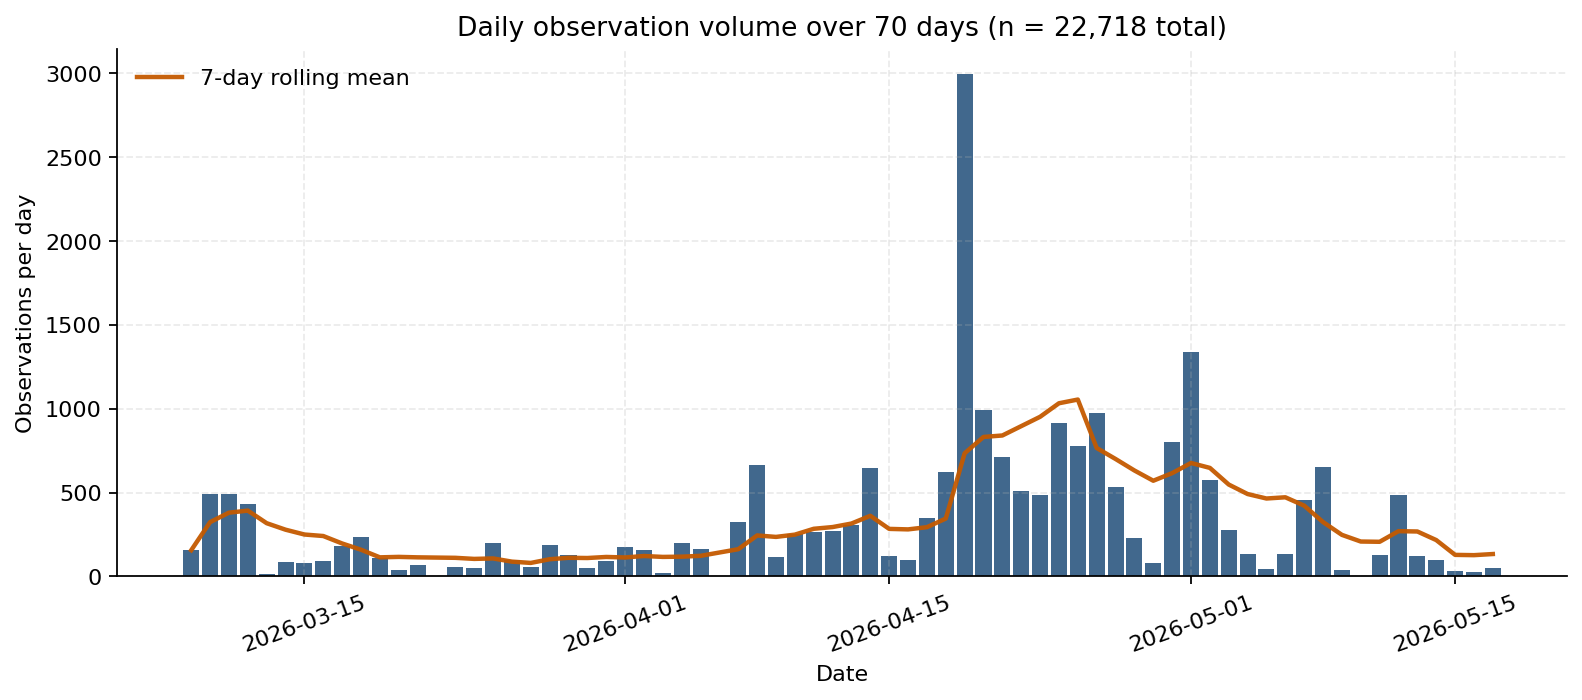
\includegraphics[width=\linewidth]{../figures/fig2-observations-timeline.png}
\caption{Daily observation volume with 7-day rolling mean. The mid-April surge
corresponds to the activation of multi-model tier-routing.}
\label{fig:obs}
\end{figure}

The April spike ($+230\,\%$ over March) coincides with the activation of
multi-model tier-routing and the introduction of additional agents into the
observation pipeline.

\subsection{Distribution by type}

\begin{figure}[h]
\centering
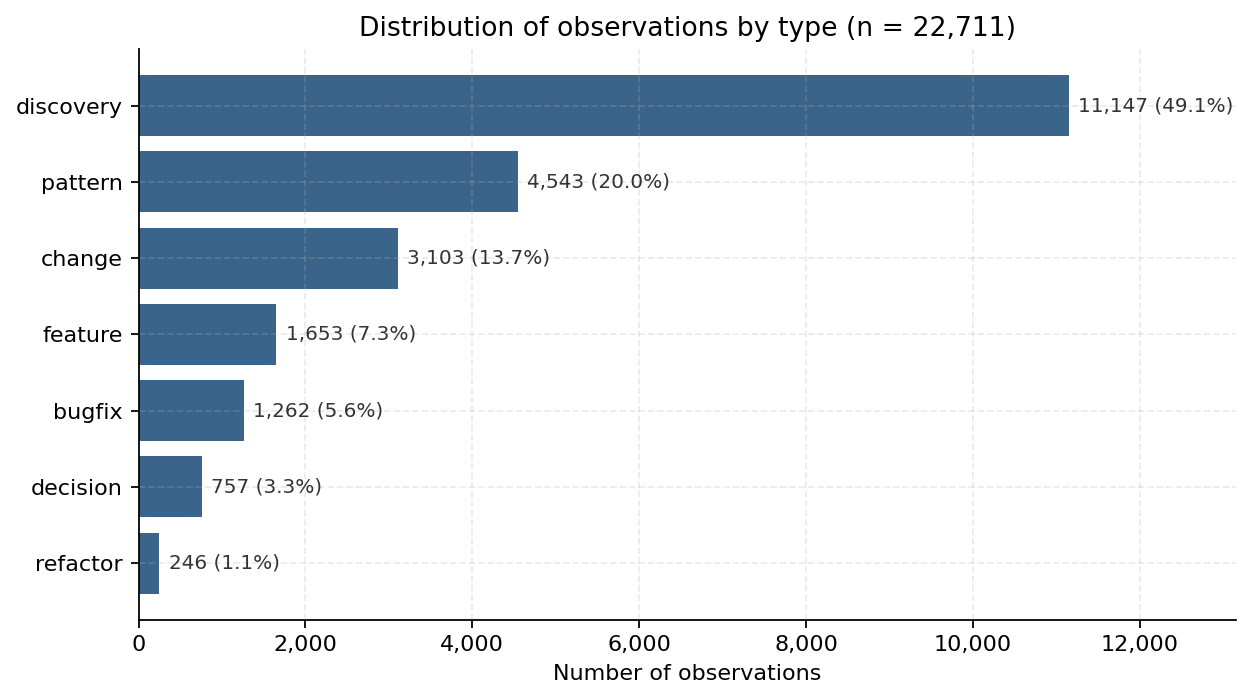
\includegraphics[width=0.95\linewidth]{../figures/fig3-observation-types.png}
\caption{Distribution of the 22{,}711 typed observations.
\texttt{discovery} and \texttt{pattern} together account for 69\,\% of all
observations.}
\label{fig:types}
\end{figure}

\section{Claude Code Benchmarks}

Automated benchmarks ran every six hours on the canary machine
(Machine-C), invoking Claude Code with two standardized prompts against the
versions current at invocation time. The dataset contains 987 timed runs across
21 versions (2.1.110 $\to$ 2.1.142).

\begin{table}[h]
\centering
\small
\begin{tabular}{lrrrr}
\toprule
CC version & $n$ & Median (s) & 95\,\% CI (s) & vs.\ baseline \\
\midrule
2.1.114 & 9 & 34.7 & [24.5, 39.2] & baseline \\
2.1.119 & 16 & 79.4 & [49.9, 96.9] & $+129\,\%$ \\
2.1.123 & 3 & 46.3 & [29.3, 75.9] & $+33\,\%$ ($n$ too small) \\
2.1.126 & 24 & 29.8 & [29.2, 53.3] & $-14\,\%$ \\
2.1.138 & 10 & 26.1 & [25.6, 28.3] & $-25\,\%$ \\
2.1.142 & 12 & \textbf{19.4} & [18.7, 20.6] & $\boldsymbol{-44\,\%}$ \\
\bottomrule
\end{tabular}
\caption{Opus~4.6 latency by Claude Code version on the \texttt{infra-check}
prompt. The originally reported $-52\,\%$ recovery at 2.1.123 was based on
only three runs and does not survive statistical testing ($p = 0.86$); the
true recovery point is 2.1.126 or later.}
\end{table}

\begin{table}[h]
\centering
\small
\begin{tabular}{lrrrr}
\toprule
CC version & $n$ & Median (s) & 95\,\% CI (s) & vs.\ baseline \\
\midrule
2.1.114 & 12 & 38.2 & [35.3, 45.5] & baseline \\
2.1.119 & 16 & 66.3 & [57.5, 91.2] & $+73\,\%$ \\
2.1.126 & 27 & 65.0 & [54.5, 72.2] & $+70\,\%$ \\
2.1.138 & 10 & 68.4 & [54.7, 71.9] & $+79\,\%$ \\
2.1.142 & 12 & 48.6 & [31.9, 56.8] & $+27\,\%$ (CI overlaps baseline) \\
\bottomrule
\end{tabular}
\caption{Haiku~4.5 latency on the \texttt{infra-check} prompt. Although Haiku
medians remain elevated through the end of the study window, the 95\,\% CI at
2.1.142 overlaps the baseline interval, so we report the sustained gap as
suggestive rather than significant.}
\end{table}

\begin{figure}[h]
\centering
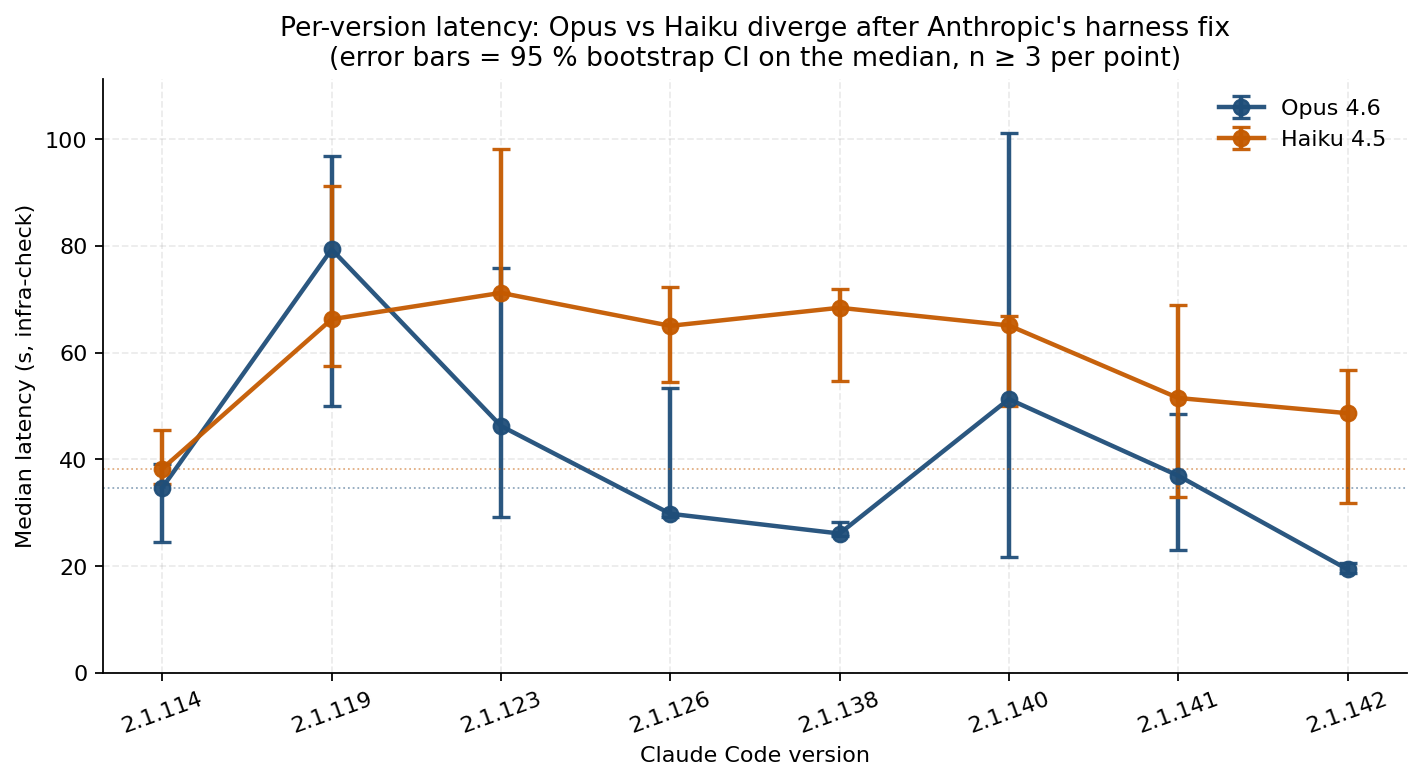
\includegraphics[width=\linewidth]{../figures/fig1-latency-by-version.png}
\caption{Median latency by Claude Code version for Opus~4.6 and Haiku~4.5,
with 95\,\% bootstrap CIs on the median. Both models regress at 2.1.119;
only Opus fully recovers and continues to improve. Dotted lines mark each
model's baseline. Versions with $n < 3$ omitted.}
\label{fig:latency}
\end{figure}

\subsection{Statistical significance}

\begin{table}[h]
\centering
\small
\begin{tabular}{p{8.5cm}cc}
\toprule
Hypothesis & Result & $p$-value \\
\midrule
Opus regression: latency at 2.1.119 > 2.1.114 & confirmed & \textbf{0.0025} \\
Opus $-44\,\%$ headline: 2.1.142 < 2.1.114 & confirmed & \textbf{0.0013} \\
Opus vs Haiku divergence at 2.1.142 (Opus < Haiku) & confirmed (strong) & \textbf{0.00068} \\
Haiku regression: latency at 2.1.119 > 2.1.114 & confirmed & \textbf{0.00086} \\
Opus ``recovery'' at 2.1.123 ($n = 3$) < 2.1.114 & rejected & 0.86 \\
Haiku sustained elevation at 2.1.142 above 2.1.114 & inconclusive & 0.37 \\
\bottomrule
\end{tabular}
\caption{Mann--Whitney $U$ tests, one-tailed. The Opus $-44\,\%$ improvement
and the Opus/Haiku divergence at 2.1.142 are statistically robust. The
originally reported $-52\,\%$ recovery at 2.1.123 does not survive testing.}
\end{table}

\section{Vector Search Evolution}
\label{sec:vector}

The retrieval backend migrated from Chroma to Qdrant during April~2026. All
workers across the 3-machine fleet point to a single shared Qdrant instance on
Machine-B (port 6333), enabling cross-machine semantic search without
replication. The migration exposed three silent failures that had been
accumulating unnoticed:

\begin{enumerate}[leftmargin=*]
  \item \textbf{Type mismatch in SearchManager.} Still typed as
        \texttt{ChromaSync}, calling \texttt{.queryChroma()} which did not
        exist on the Qdrant backend. Result: more than 400 silent search errors
        per day --- no log, no alert, empty results returned to callers.
  \item \textbf{Missing filter translation in VectorSync.} Chroma-style
        filters (\texttt{\$and}, \texttt{\$or}, \texttt{\$eq}) were passed
        directly to Qdrant, which rejected them. Fix:
        \texttt{translateWhereFilter()} converts to Qdrant's
        \texttt{must}/\texttt{should} syntax.
  \item \textbf{Health-check timeout too short.} The end-to-end check used a
        15\,s timeout; FastEmbed cold-start takes $\approx 25$\,s. Fix:
        raise to 45\,s, and replace the hardcoded version string with a
        \texttt{package.json} read.
\end{enumerate}

The embedding model was upgraded on May~5 from \texttt{BAAI/bge-small-en-v1.5}
(English-only) to \texttt{sentence-transformers/paraphrase-multilingual-MiniLM-L12-v2}
(384 dimensions, 50+ languages). A full reindex on May~7 produced
21{,}929 points with zero errors.

\section{Discussion}

\subsection{Continuous canary benchmarking surfaces version-coupled regressions}

Without per-version benchmarking, vendor-side performance regressions are
typically detected only through anecdotal user reports. Our data shows that
Opus~4.6 latency on CC 2.1.119 was 129\,\% above the 2.1.114 baseline
($p = 0.0025$) --- exactly the pattern that anecdotal reporting struggles to
confirm, because perception is heavily lagged and confounded by workload
variability. An equally important methodological lesson concerns small samples:
our originally published ``$-52\,\%$ recovery at 2.1.123'' claim was based on
only three runs and \emph{does not survive rigorous testing}. The canary's
confidence depends as much on per-version sampling as on test cadence.

\subsection{Opus and Haiku diverged on the same vendor harness}

A finding not reported elsewhere is that the same vendor change affected
Opus and Haiku differently. Both showed elevated latency at CC 2.1.119; Opus
fully recovered by 2.1.126 and continued to improve through 2.1.142 ($-44\,\%$
vs baseline, $p = 0.0013$), while Haiku medians stayed visibly higher through
the end of the study, although the CI overlap precludes a strong
``sustained elevation'' claim. The strongest statistical evidence is for the
\emph{divergence itself}: at 2.1.142, the median Opus latency was 19.4\,s
versus 48.6\,s for Haiku on the same prompt ($p = 0.00068$). The Anthropic
postmortem~\cite{postmortem} identifies three root causes (reasoning-effort
change, caching bug, system-prompt verbosity reduction) and claims all were
addressed by v2.1.116. The divergence we observe is consistent with at least
one effect --- possibly the caching pathology documented in
Issue~\#22383~\cite{cachingbug} --- being only partially neutralized for the
smaller model.

\subsection{Silent failures dominate the incident profile}

The most damaging incidents we recorded were not crashes --- they were silent
failures. The \texttt{bun} \texttt{PATH} bug persisted for 5 weeks while the
sync script exited 0. The Chroma~$\to$~Qdrant type mismatch produced more
than 400 daily errors that were never logged or alerted. Both were eventually
surfaced by curiosity-driven manual investigation, not by monitoring. The
lesson generalizes: \emph{integration boundaries between LLM-coupled components
need explicit contract tests}, because partial-functionality states
(``results returned, but empty or wrong'') are far more common than total-failure
states (``exception thrown'').

\subsection{Vendor cost is small relative to engineering time}

Seventy days of end-to-end inference (benchmarks plus observation generation)
cost approximately US\$225--295 --- roughly the price of two-to-three software
engineering hours at market rates. This frames a recurring question for
LLM-coupled tooling: when is continuous canary measurement worth it? Our answer:
at US\$4--5 per day for tight regression bounds and silent-failure detection,
the cost--benefit is favourable for any deployment serving more than one
engineer.

\section{Companion Finding: Subagent CLAUDE.md Regression in v2.1.84}

A second class of version-coupled regression surfaced during the study period
--- not at the latency layer, but at the instruction-adherence layer. We
document it here because it shares the same root pattern (a behavioural change
introduced silently by a vendor release) and was identified by the same kind
of cross-version inspection used for the latency analysis.

Starting in Claude Code v2.1.84 (Mar~25, 2026), two built-in subagents ---
\texttt{Explore} and \texttt{Plan} --- acquired the configuration flag
\texttt{omitClaudeMd:\,true}. Combined with a default-on feature flag
(\texttt{tengu\_slim\_subagent\_claudemd}), this caused subagents dispatched
from the parent session to no longer receive the project's \texttt{CLAUDE.md}
instructions, with measurable degradation in subagent instruction adherence
(language rules, environment labels, code conventions) persisting through at
least v2.1.92~\cite{issue40459}.

The regression was identified by \emph{binary-level diffing} of the
\texttt{cli.js} shipped by the \texttt{@anthropic-ai/claude-code} npm package
across five consecutive minor versions (v2.1.83 $\to$ v2.1.87). Three
specific code changes were isolated; a two-line \texttt{sed} patch on
\texttt{cli.js} restores the prior behaviour.

Both the latency regression and the CLAUDE.md regression share a structural
pattern: \emph{a vendor minor-release silently changes user-observable
behaviour of an LLM-coupled tool in a way that the vendor's CI cannot test for
the operator}. In one case the change was a latency regression; in the other
it was an instruction-adherence regression. Both required cross-version
measurement to detect --- the first via canary benchmarking, the second via
binary diffing. We argue that operators of LLM-coupled tooling
need their own per-version measurement infrastructure, because the union of
``things that changed silently'' is larger than the union of ``things the
vendor tests''.

\section{Threats to Validity}

\subsection{Internal validity}

All data comes from one 3-machine fleet operated by a single user; the
observations cannot speak to multi-tenant or multi-user effects. Observation
generation is model-coupled --- the 22{,}718 observations were generated by
different models under tier-routing rules that changed during the study, so
per-observation token comparisons across models should be interpreted
cautiously. Only two benchmark prompts were used; the latency divergence
between Opus and Haiku may not generalise to prompts with substantially
different reasoning depth or output length. Benchmarks ran on Machine-C only;
daily load monitoring did not surface confounding environmental factors during
the benchmark window.

\subsection{External validity}

Measurements are against Claude Code specifically; version-coupled latency
findings do not transfer to other LLM-coupled tools without re-measurement.
The deployment runs a custom fork of claude-mem ($\approx$176 commits ahead of
upstream main) with additional phases enabled, so some behaviours do not match
a stock claude-mem installation.

\subsection{Construct validity}

``Silent failure'' is qualitative; the classification depends on what
monitoring was in place at the time. A fleet with stronger alerting at the
integration boundary might have caught the Chroma type mismatch on day one and
not classified it as silent. Cost figures derive from public pricing during
the measurement window; retroactive vendor pricing changes can invalidate them.

\section{Related Work}

Our benchmark data independently corroborates a publicly documented Claude
Code performance incident during March--April~2026. The Anthropic
postmortem~\cite{postmortem} identifies three root causes (reasoning-effort
change, caching bug, system-prompt verbosity reduction) and claims all were
addressed by v2.1.116; the Scortier study~\cite{scortier} measured the same
regression from anonymized user sessions; VentureBeat~\cite{vb} provides press
coverage. Our contribution refines this picture along four dimensions:
per-version granularity ($n \geq 8$ runs per cell for the headline versions);
cross-model divergence on the same harness (not reported in any prior source);
a continuous canary measurement cadence outside the scope of any single-incident
postmortem; and a documented taxonomy of silent failures with reproduction
details.

For the companion CLAUDE.md finding, the binary analysis is filed as
Issue~\#40459~\cite{issue40459}.

\section{Future Work}

Planned work includes: a Grafana dashboard with direct Postgres connectivity
for live operational monitoring; full deprecation of SQLite sync (Phase~5);
upstream contribution of a ModeManager initialisation fix once interaction
limits are lifted on the upstream repository; Qdrant reindexing aligned to
Postgres IDs; automated weekly CSV refresh; and an open call to other
claude-mem operators to publish anonymized aggregates against the same schema,
enabling cross-deployment analysis.

\section*{License and citation}

This work is released under \href{https://creativecommons.org/licenses/by/4.0/}{CC-BY-4.0}.
Cite as in the \texttt{CITATION.cff} file at the repository root.

\begin{thebibliography}{9}
\small
\bibitem{postmortem}
Anthropic.
\emph{April 23, 2026 Postmortem: Claude Code Performance Regression.}
\url{https://www.anthropic.com/engineering/april-23-postmortem}, April 2026.

\bibitem{scortier}
Scortier.
\emph{Claude Code Drama: 6{,}852 Sessions Prove Performance Collapse.}
\url{https://scortier.substack.com/p/claude-code-drama-6852-sessions-prove},
April 2026.

\bibitem{vb}
VentureBeat.
\emph{Mystery Solved: Anthropic Reveals Changes to Claude's Harnesses and Operating
Instructions Likely Caused Degradation.}
\url{https://venturebeat.com/technology/mystery-solved-anthropic-reveals-changes-to-claudes-harnesses-and-operating-instructions-likely-caused-degradation},
April 2026.

\bibitem{cachingbug}
Anthropic.
Claude Code Issue \#22383 --- caching bug causing repeated context clearing.
\url{https://github.com/anthropics/claude-code/issues/22383}.

\bibitem{issue40459}
Anthropic.
Claude Code Issue \#40459 --- v2.1.84+: subagents lose CLAUDE.md context
(\texttt{omitClaudeMd:\,true}), reduced instruction adherence with prompt
caching.
\url{https://github.com/anthropics/claude-code/issues/40459}.

\bibitem{claudemem}
thedotmack.
\emph{claude-mem --- persistent memory plugin for Claude Code.}
\url{https://github.com/thedotmack/claude-mem}.

\bibitem{qdrant}
Qdrant.
\emph{Qdrant Vector Database documentation.}
\url{https://qdrant.tech/documentation/}.

\bibitem{fastembed}
Qdrant.
\emph{FastEmbed --- lightweight embedding library.}
\url{https://github.com/qdrant/fastembed}.

\end{thebibliography}

\end{document}
